
\begin{frame}
  \frametitle{Neural Network}
  \centering
\newcommand{\inputnum}{4}

% Hidden layer neurons'number
\newcommand{\hiddennumA}{5}
\newcommand{\hiddennumB}{6}

% Output layer neurons'number
\newcommand{\outputnum}{4}

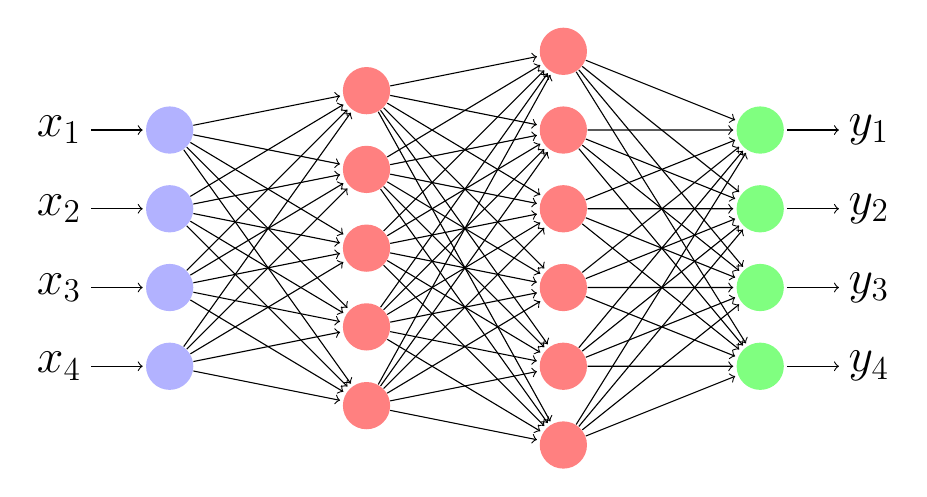
\begin{tikzpicture}


% Input Layer
\foreach \i in {1,...,\inputnum}
{
	\node[circle,
		minimum size = 6mm,
		fill=blue!30] (Input-\i) at (0,-\i) {};
}

% Hidden Layer1
\foreach \i in {1,...,\hiddennumA}
{
	\node[circle,
		minimum size = 6mm,
		fill=red!50,
		yshift=(\hiddennumA-\inputnum)*5 mm
	] (Hidden1-\i) at (2.5,-\i) {};
}

% Hidden Layer2
\foreach \i in {1,...,\hiddennumB}
{
	\node[circle,
		minimum size = 6mm,
		fill=red!50,
		yshift=(\hiddennumB-\inputnum)*5 mm
	] (Hidden2-\i) at (5,-\i) {};
}

% Output Layer
\foreach \i in {1,...,\outputnum}
{
	\node[circle,
		minimum size = 6mm,
		fill=green!50,
		yshift=(\outputnum-\inputnum)*5 mm
	] (Output-\i) at (7.5,-\i) {};
}

% Connect neurons In-Hidden
\foreach \i in {1,...,\inputnum}
{
	\foreach \j in {1,...,\hiddennumA}
	{
		\draw[->, shorten >=1pt] (Input-\i) -- (Hidden1-\j);
	}
}

% Connect neurons In-Hidden
\foreach \i in {1,...,\hiddennumA}
{
	\foreach \j in {1,...,\hiddennumB}
	{
		\draw[->, shorten >=1pt] (Hidden1-\i) -- (Hidden2-\j);
	}
}

% Connect neurons Hidden-Out
\foreach \i in {1,...,\hiddennumB}
{
	\foreach \j in {1,...,\outputnum}
	{
		\draw[->, shorten >=1pt] (Hidden2-\i) -- (Output-\j);
	}
}

% Inputs
\foreach \i in {1,...,\inputnum}
{
	\draw[<-, shorten <=1pt] (Input-\i) -- ++(-1,0)
		node[left]{\LARGE{$x_{\i}$}};
}

% Outputs
\foreach \i in {1,...,\outputnum}
{
	\draw[->, shorten <=1pt] (Output-\i) -- ++(1,0)
		node[right]{\LARGE{$y_{\i}$}};
}

\end{tikzpicture}
\end{frame}
